\section{Satellite control}

\begin{itemize}
    \item[-] \textbf{Draw the (detailed) control loop of the proposed control system, and precise which data you will pass at the interfaces between the boxes representing the control system. }

    \begin{figure}[h]
        \centering
        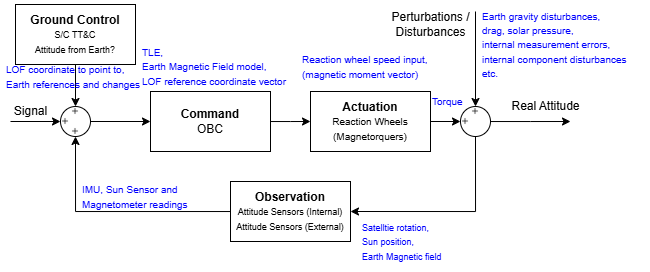
\includegraphics[width=\linewidth]{Doc/Graphics/AOCS control loop.png}
        \caption{AOCS control loop with data passing indicated in blue }
        \label{fig:enter-label}
    \end{figure}
    
    \item[-] \textbf{What is the data that you need to compute on-board and what is the data that you need to give to the satellite from the ground? }

    \textbf{On-Board Data:}
    Since no information was given on what the CubeSat would point to (and measure) I have to assume that pointing needs to be possible at any stage in the orbit. 
    As such, the CubeSat shall be able to operate semi-independently of ground control, as having ground stations available for continuous CubeSat monitoring and command can be tedious and costly. 
    Any changes to the CubeSat modes would thus be made only when the CubeSat would be in range to the main Ground Station and the precise attitude of the CubeSat would need to be calculated on-board based off the two external sensor readings. 
    Also the control for the actuation would need to be computed onboard based on the data from the internal attitude measurements.

    
    \textbf{Ground Data:}
    From the ground we would at least need to give the TT\&C commands to change the CubeSat to pointing mode and possibly to a correction mode for offloading the reaction wheels with the magnetorquers. 
    The Earth Magnetic Field model should also be updated regularly to the CubeSat from ground in addition to any corrections to the satellite's attitude as compared to the perceived attitude from Earth.

    The desired attitude, as a LOF vector and durations for pointing would also need to be updated from the ground.
    
\end{itemize}